%% Copernicus Publications Manuscript Preparation Template for LaTeX Submissions
%% ---------------------------------
%% This template should be used for copernicus.cls
%% The class file and some style files are bundled in the Copernicus Latex Package, which can be downloaded from the different journal webpages.
%% For further assistance please contact Copernicus Publications at: production@copernicus.org
%% https://publications.copernicus.org/for_authors/manuscript_preparation.html


%% Please use the following documentclass and journal abbreviations for preprints and final revised papers.

%% 2-column papers and preprints
\documentclass[essd, manuscript]{copernicus}



%% Journal abbreviations (please use the same for preprints and final revised papers)


% Advances in Geosciences (adgeo)
% Advances in Radio Science (ars)
% Advances in Science and Research (asr)
% Advances in Statistical Climatology, Meteorology and Oceanography (ascmo)
% Annales Geophysicae (angeo)
% Archives Animal Breeding (aab)
% ASTRA Proceedings (ap)
% Atmospheric Chemistry and Physics (acp)
% Atmospheric Measurement Techniques (amt)
% Biogeosciences (bg)
% Climate of the Past (cp)
% DEUQUA Special Publications (deuquasp)
% Drinking Water Engineering and Science (dwes)
% Earth Surface Dynamics (esurf)
% Earth System Dynamics (esd)
% Earth System Science Data (essd)
% E&G Quaternary Science Journal (egqsj)
% European Journal of Mineralogy (ejm)
% Fossil Record (fr)
% Geochronology (gchron)
% Geographica Helvetica (gh)
% Geoscience Communication (gc)
% Geoscientific Instrumentation, Methods and Data Systems (gi)
% Geoscientific Model Development (gmd)
% History of Geo- and Space Sciences (hgss)
% Hydrology and Earth System Sciences (hess)
% Journal of Bone and Joint Infection (jbji)
% Journal of Micropalaeontology (jm)
% Journal of Sensors and Sensor Systems (jsss)
% Magnetic Resonance (mr)
% Mechanical Sciences (ms)
% Natural Hazards and Earth System Sciences (nhess)
% Nonlinear Processes in Geophysics (npg)
% Ocean Science (os)
% Polarforschung - Journal of the German Society for Polar Research (polf)
% Primate Biology (pb)
% Proceedings of the International Association of Hydrological Sciences (piahs)
% Scientific Drilling (sd)
% SOIL (soil)
% Solid Earth (se)
% The Cryosphere (tc)
% Weather and Climate Dynamics (wcd)
% Web Ecology (we)
% Wind Energy Science (wes)


%% \usepackage commands included in the copernicus.cls:
%\usepackage[german, english]{babel}
%\usepackage{tabularx}
%\usepackage{cancel}
%\usepackage{multirow}
%\usepackage{supertabular}
%\usepackage{algorithmic}
%\usepackage{algorithm}
%\usepackage{amsthm}
%\usepackage{float}
%\usepackage{subfig}
%\usepackage{rotating}


\begin{document}

\title{Nearshore surface wave dynamics and kinematics measurements from arrays of ‘microSWIFT’ drifters}


% \Author[affil]{given_name}{surname}

\Author[University of Washington, Applied Physics Laboratory]{EJ}{Rainville}
\Author[University of Washington, Applied Physics Laboratory]{Jim}{Thomson}
\Author[University of Washington, Applied Physics Laboratory]{Melissa}{Moulton}
\Author[University of Washington, Applied Physics Laboratory]{Morteza}{Derakhti}

\affil[University of Washington, Applied Physics Laboratory]{ADDRESS}

%% The [] brackets identify the author with the corresponding affiliation. 1, 2, 3, etc. should be inserted.

%% If an author is deceased, please mark the respective author name(s) with a dagger, e.g. "\Author[2,$\dag$]{Anton}{Aman}", and add a further "\affil[$\dag$]{deceased, 1 July 2019}".

%% If authors contributed equally, please mark the respective author names with an asterisk, e.g. "\Author[2,*]{Anton}{Aman}" and "\Author[3,*]{Bradley}{Bman}" and add a further affiliation: "\affil[*]{These authors contributed equally to this work.}".


\correspondence{EJ Rainville (erainvil@uw.edu)}

\runningtitle{TEXT}

\runningauthor{TEXT}




\received{}
\pubdiscuss{} %% only important for two-stage journals
\revised{}
\accepted{}
\published{}

%% These dates will be inserted by Copernicus Publications during the typesetting process.


\firstpage{1}

\maketitle



\begin{abstract}
TEXT
\end{abstract}


\copyrightstatement{TEXT} %% This section is optional and can be used for copyright transfers.

\seection{Figure List}
Figure \ref{fig:1}
Figure \ref{fig:2}



\introduction  %% \introduction[modified heading if necessary]
Free-floating drifters are used to measure properties of the ocean in a Lagrangian framework. However, we generally care about the ocean in an Eulerian or fixed frame perspective compared to a moving frame. Many properties of the ocean have been measured using drifters including sea surface temperature, salinity and surface velocity. The sea surface elevation is difficult to measure directly and typically is computed from other indirect measurements such as accelerations or velocities in combination with a theoretical framework for how the surface moves using those kinematic measurements. Furthermore, measuring the sea surface elevation in shallow water can be even more challenging due to the nonlinear nature of the sea surface motion. Considering that many people live near the coasts, we care deeply about the dynamics of the coasts. The defining characteristic of coastal hydrodynamics is the transformation of deep water waves to shallow water waves and eventually to wave breaking that leads to turbulence, mixing and sediment transport. Water wave breaking has been studied for a long time; however, due to the complex nature of measuring the nearshore environment due to high loads and complex flows most theory and modeling must be reduced to statistical comparisons between models and measurements or reduced to one dimensional models that miss the along shore variability of the nearshore environment. Remote sensing techniques such as LiDAR and camera rectification techniques allow us to measure things such as the slope of the wave and an estimate of the elevation; we are not able to get direct in situ measurements of the accelerations and velocities on the surface. Understanding the transformation of the waves from deep water waves to shallow water waves helps us to understand when waves will break and how much energy is dissipated in the process. 


\section{Measurements}
During October 2021, a 27 day field campaign was held where coherent arrays of small-scale drifters were deployed daily into the nearshore environment. The site of this study was the US Army Corps of Engineers Field Research Facility in Duck, North Carolina, USA. The goal of the project was to obtain in-situ measurements of the accelerations, velocities and sea surface elevations with high spatial and temporal resolution from drifters. Fixed instrumentation at the field site included Argus imagery, water level gauges, offshore wave buoys and high resolution bathymetry surveys conducted by the Field Research Facility. The combination of all these instruments will help to understand more about the dynamics of the nearshore environment with a special emphasis on large wave events as this project was part of the larger collaborative DUNEX(DUring Nearshore Events eXperiment) project.

\subsection{The microSWIFT}
The small-scale, free-drifting wave buoys used in this study are called microSWIFTs and are shown in Figure \ref{fig:1}. 
\begin{figure}
    \centering
    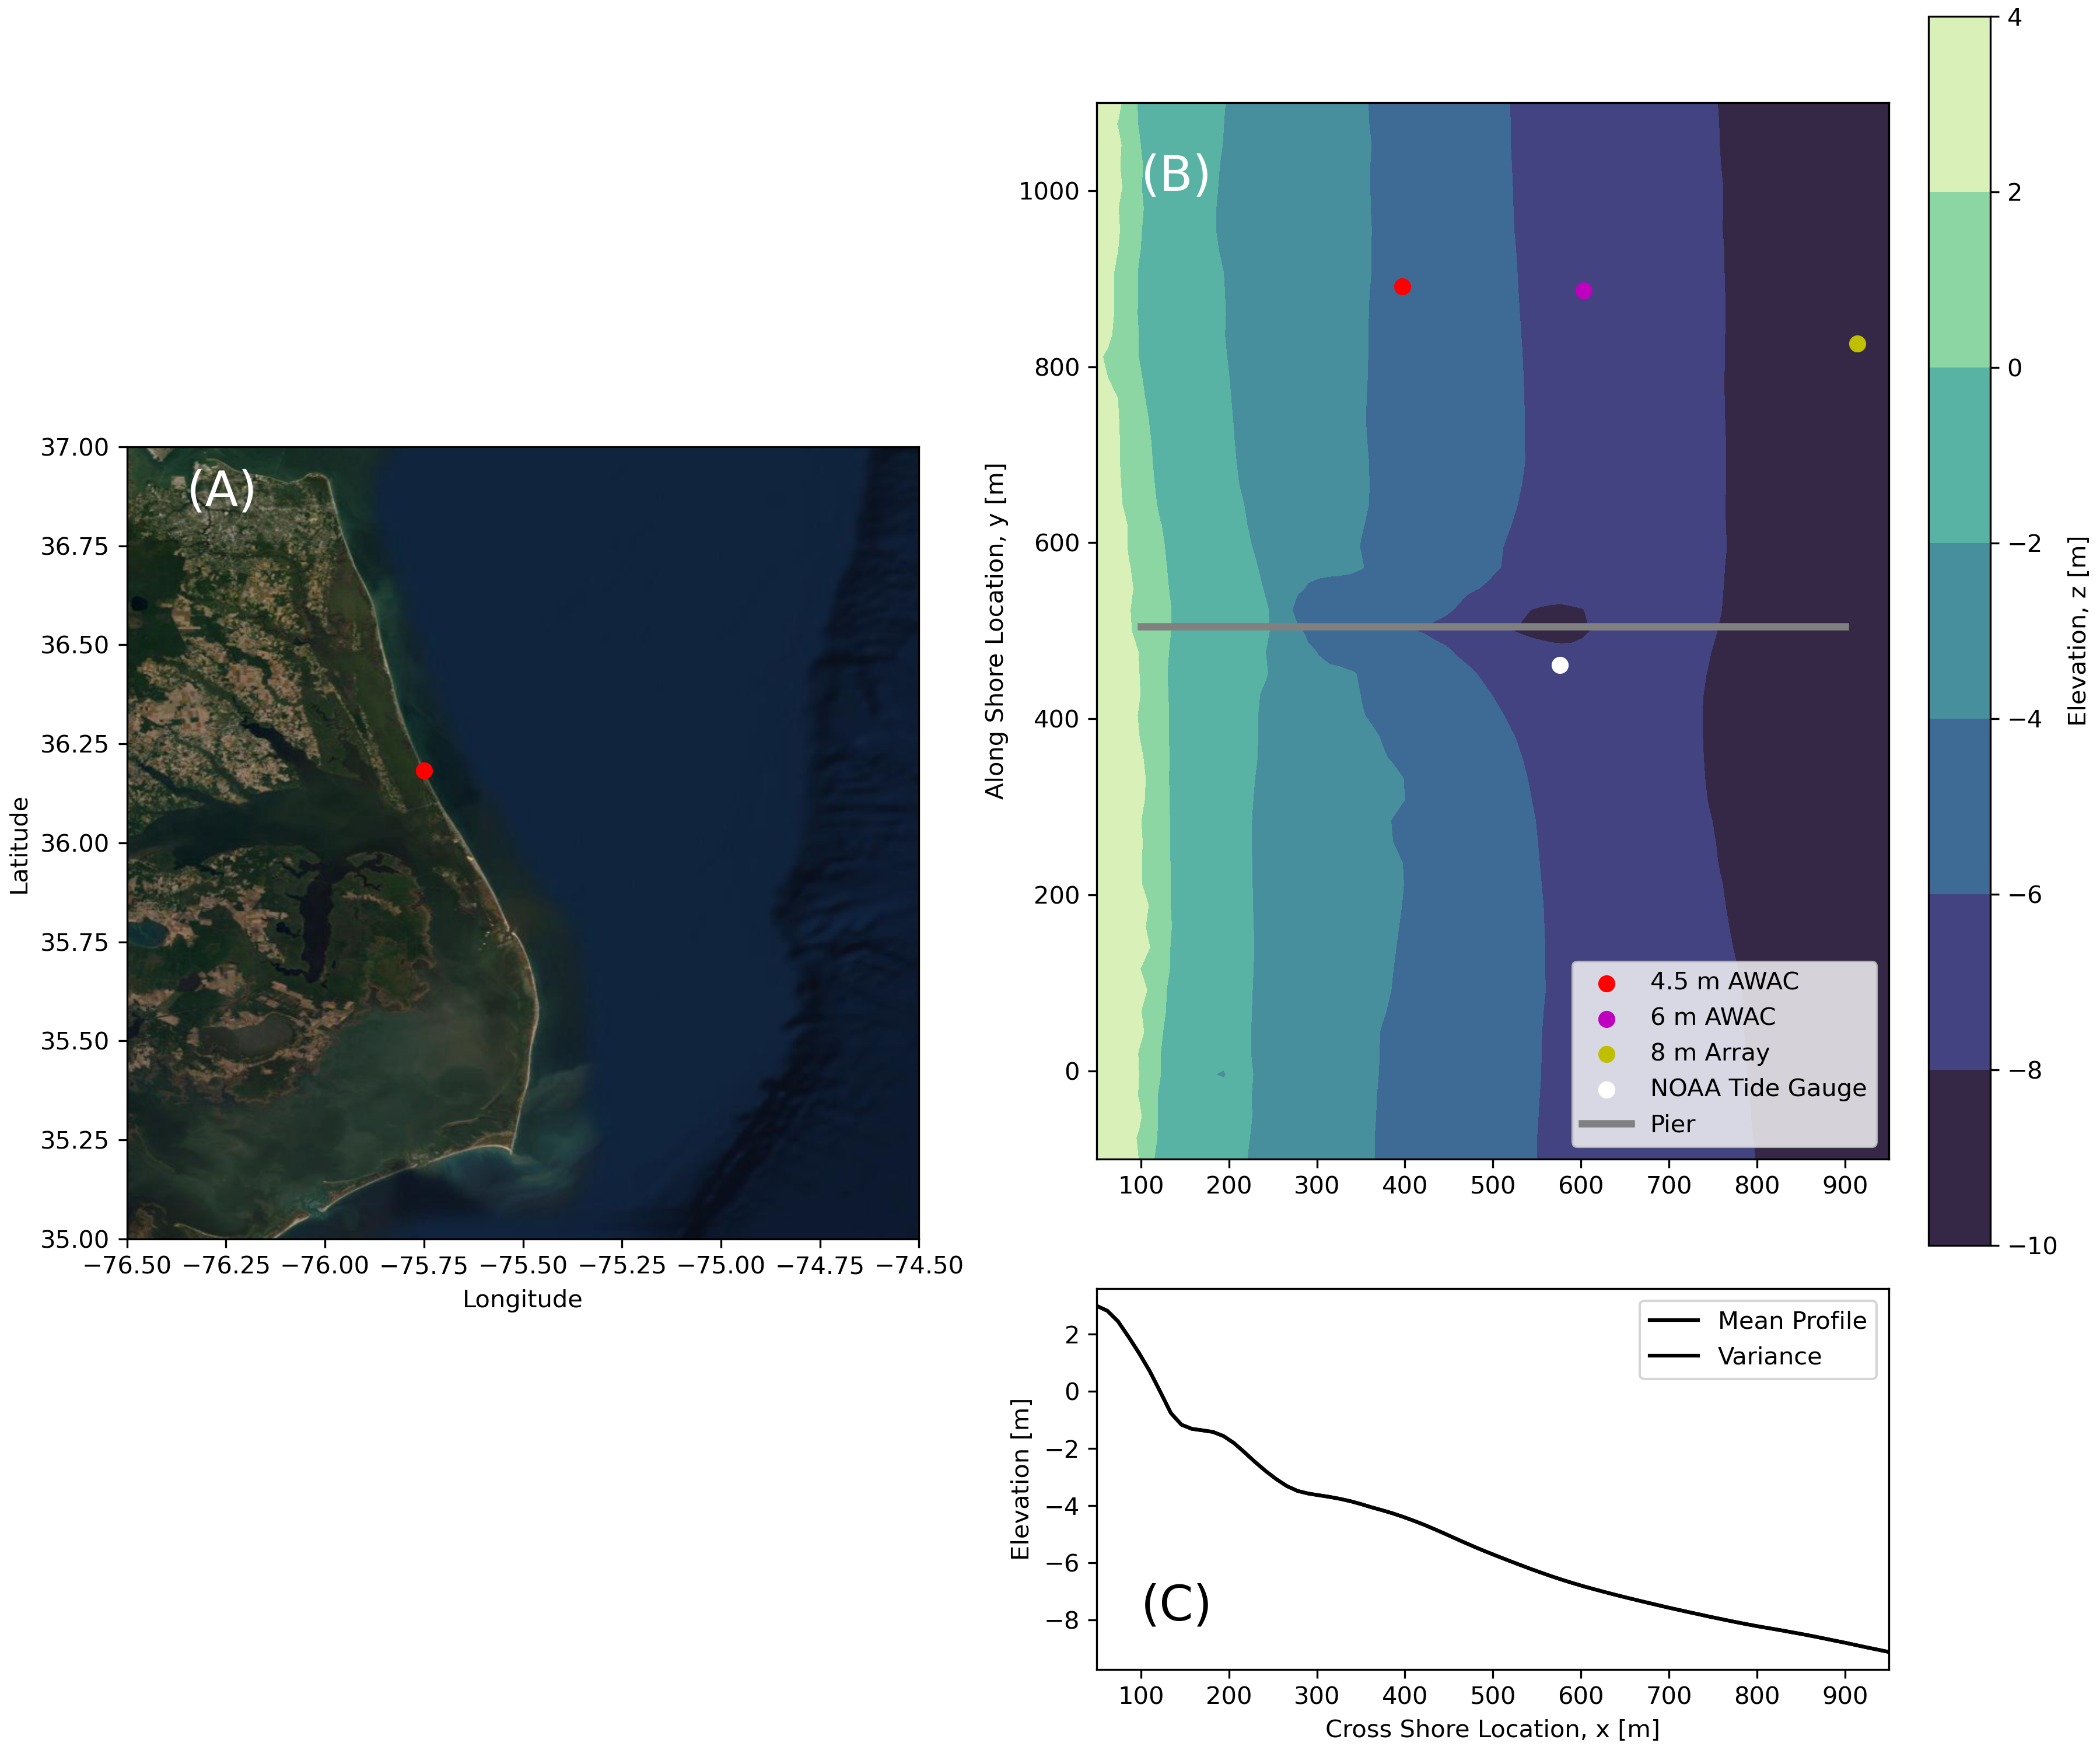
\includegraphics[width=\textwidth,height=\textheight,keepaspectratio]{Figures/fig01.png}
    \caption{Layout of main components in the microSWIFT Buoys. Housing is Nalgene water bottle, battery chassis and main body circuit board. The main body is controlled by a raspberry pi micro-controller has an IMU and GPS module for measurements and an Iridium modem to transmit data. }
    \label{fig:1}
\end{figure}

The microSWIFT is an extension from the original SWIFT (Surface Wave Instrument Float with Tracking) that is described in \citeauthor{thomson_wave_2012} \citeyear{thomson_wave_2012}. The microSWIFT is housed inside of a Nalgene brand water bottle with a length of approximately 21 cm and a diameter of 9 cm. The bottle sits on its side on the water giving a keel of approximately 4.5 cm and a sail of 4.5 cm. The overall microSWIFT has a mass of approximately 0.7 kg. The instruments on board the microSWIFT are a GPS module and Inertial Measuremesnt Unit (IMU). The GPS Module uses the MT3339 chipset with a sensitivity of -165dBm. The GPS Samples at a rate of 4 Hz and reads direct NMEA strings. We read in the GPGGA and GPVTG NMEA strings which give measurements of the buoy position(latitude and longitude), altitude, speed over ground and course over ground. The course over ground is used to break the speed over ground up into East-West an North-South velocity components. The position and velocity measurements are then transformed into a local Cartesian coordinate system for that has been established for the Field Research Facility. The IMU on board incorporates an accelerometer, gyroscope and magnetometer integrated onto one chip all that measure in 3 orthogonal directions. The specifications for the IMU are stated in Table \ref{table:1}.

\begin{table}[h!]
    \centering
    \begin{tabular}{cccccc}
        \hline
        Sensor & Chip & Sensitivity & Dynamic Range & Noise Density \\
        \hline
        3-axis Linear Accelerometer & FXOS8700CQ & 0.244 mg/LSB / 0.488 mg/LSB & \pm 2g / \pm 4g  &  < 126 μg/√Hz (200-Hz bandwidth) \\
        3-axis Magnetometer & FXOS8700CQ & 0.1 \mu T/LSB & \pm 1200 \mu T & < 100 nT/√Hz (100-Hz bandwidth)\\ 
        3-axis Gryoscope & FXAS21002C &  15.625 mdps/LSB & \pm 500 dps & 25 mdps/√Hz (64 Hz bandwidth)\\
        \hline
        \\ \bottomrule
    \end{tabular}
    \caption{Inertial Measurement Unit sensor specifications for accelerometer, gyroscope and magnetometer onboard each microSWIFT. }
    \label{table:1}
\end{table}

Deployments of coherent drifter arrays were referred to as "missions" in the context of this experiment. The microSWIFTs were deployed by personnel swimming them out on surfboards, thrown from the Field Research Facility pier, taken out by jet-ski from local lifeguards and dropped from a helicopter. It is important to note that the microSWIFTs deployed from the helicopter had parachutes attached and therefore may act hydrodynamically different than the other microSWIFTs. Many of the missions lasted approximately 20 minutes while some are shorter and few go longer than an hour. A total of 81 missions were completed during the experiment with some of those missions being removed from the overall cleaned dataset mostly due to being too short all which have been noted in a description sheet attached with the dataset.

The microSWIFT is controlled by a Raspberry Pi Zero micro-controller which schedules recording, on board processing and data sending windows based on a time schedule. The microSWIFT systems initialize all sensors at the start of every hour in UTC time. The microSWIFT then records data from the IMU and GPS sensors at sampling rates of 12 Hz and 4 Hz, respectively until minute 50 of the hour is reached. Once the recording window is ended, the microSWIFT processes some of the data and sends the data via iridium telemetry through an on-board iridium modem(RockBLOCK 9603) to a local server. This feature was not heavily utilized in this project but will be more relevant in future deep water projects. The dataset has been quality controlled through a uniform processing method that is described in the following data processing section.

\subsection{Conditions and Area Sampled}
We were able to obtain a rich dataset of many wave and atmospheric conditions using the combination of the microSWIFT coherent arrays and the permanent instruments at the Field Research Facility. The conditions that were sampled are shown in Figure \ref{fig:2}.

\begin{figure}
    \centering
    \includegraphics{}
    \caption{Distributions of  }
    \label{fig:2}
\end{figure}

During this experiment we deployed arrays of microSWIFTs 

Throughout the overall experiment, we deployed a total of 2,187 buoys into the ocean and retrieved all but one of the buoys. The area that was covered by drifter deployments over the course of the entire experiment is shown in Figure \ref{composite_map}. 

\begin{figure}
    \centering
    \includegraphics{}
    \caption{Composite map of all drifter locations throughout the entire experiment. The solid black line shows the boundaries of typical bathymetry surveys. The coordinate system is a local Cartesian coordinate system developed by the Field Research Facility. }
    \label{fig:composite_map}
\end{figure}
 
The area covered was generally from just outside of the surfzone and to the swash zone. The microSWIFT arrays were deployed with the intent to stay within the area that has regular bathymetry surveys to compare the wave measurements with. If the drifters were heading offshore, they were picked up using various methods raging from swimmers to people on jet-skis depending on available resources. The times when the buoys were not free drifting have been cleaned from the data set as will be described more thoroughly in section 3a. 

\section{Data Processing}
 The raw data channels from the microSWIFTs give measurements of the latitude, longitude, GPS elevation, course over ground, speed over ground, accelerations, rotations and current heading all to varying degrees of accuracy as described in Table \ref{table:1}.
 The data is organized on a "mission" based system which means that each array that was deployed was referred to as a "mission." Each microSWIFT that was deployed in the array is written down prior to deployment so that the number that went out and the numbers of each microSWIFT can be kept track of in combination with the mission number. Upon deploying the microSWIFTs, a "start" time is written in UTC time. Once all of the microSWIFTs were collected back on the beach an "end" time for the mission was recorded by hand. Using the mission numbers, microSWIFTs on the mission, start and end times we are able to organize the raw data into coherent datasets. After this initial organization, the data from each microSWIFT array is processed uniformly in the following procedure. First, the raw data is in text files, so it is parsed and converted to numeric values. The timestamps from each measurement are then organized between the start and end times of the mission. The corresponding data that are within the bounds are kept and sorted to be increasing in time. The IMU sensors samples at a rate of 12 Hz while the GPS samples at a rate of 4 Hz. Therefore to have a uniform time array, the GPS values are linearly interpolated onto the 12 Hz sampling rate. Once a uniform time array is generated, any missing data points from any channel are filled via a linear interpolation method. Once the data is organized into missions and sorted onto one time array so that it can be indexed uniformly, a spatial mask is created to remove any data points while it is on the beach. This mask is created using bathymetric surveys conducted at the Field Research Facility and the mean water level during the mission in question. The furthest point offshore that is computed to be dry land from adding the mean water level to the bathymetric survey is used as a threshold to remove any data points further onshore than this line. An additional buffer is added to the spatial threshold of 5 meters just to ensure that any points offshore of this line are definitely in the water. So any points that 

Details of the state estimator are described in section 3b below.  In order to make a cohesive data set, an overall time vector is developed for the entire length of the mission with a time step equal to that of the IMU sampling rate of 1/12 of a second. The IMU measurements from each microSWIFT are then matched indices within this overall time array using a binary search algorithm. The GPS data that is sampled at a slower rate is then linearly interpolated onto the overall time array. Now that all measurements are on the same set of indices and time points, the data can be cleaned for valid and invalid data. For the purposes of this experiment, invalid data is defined as any time the microSWIFT is not floating freely on the surface of the ocean. While this may seem like an easy task to screen through, due to the highly varied nature of the deployment methods and the highly variable conditions of the nearshore environment sometimes the microSWIFTs would be picked up if they were drifting offshore and 


The GPS measurements are in the earth frame of reference and can be directly converted to the local FRF coordinate system. However, the IMU measurements are within the frame of reference of the drifter and with the exception of the heading measurements, the drifter is agnostic to the Earth frame of reference. 

\section{Data Products and Validation}
In order to make the data from the coherent arrays of drifters useful, the data must be organized and cleaned then converted into useful data products for further analysis. The general outline of this process is removing invalid data, interpolating the GPS data onto the IMU sampling frequency, computing best state estimates of the drifter and then gridding that data into a spatial grid

What can we do with these measurements:
\begin{list}
    \item Track location of breakers - this is pretty huge and new! (Use in conjunction with 
\end{list}

\conclusions  %% \conclusions[modified heading if necessary]
TEXT

%% The following commands are for the statements about the availability of data sets and/or software code corresponding to the manuscript.
%% It is strongly recommended to make use of these sections in case data sets and/or software code have been part of your research the article is based on.

\codeavailability{TEXT} %% use this section when having only software code available


\dataavailability{TEXT} %% use this section when having only data sets available


\codedataavailability{TEXT} %% use this section when having data sets and software code available


\sampleavailability{TEXT} %% use this section when having geoscientific samples available


\videosupplement{TEXT} %% use this section when having video supplements available


\appendix
\section{}    %% Appendix A

\subsection{}     %% Appendix A1, A2, etc.


\noappendix       %% use this to mark the end of the appendix section. Otherwise the figures might be numbered incorrectly (e.g. 10 instead of 1).

%% Regarding figures and tables in appendices, the following two options are possible depending on your general handling of figures and tables in the manuscript environment:

%% Option 1: If you sorted all figures and tables into the sections of the text, please also sort the appendix figures and appendix tables into the respective appendix sections.
%% They will be correctly named automatically.

%% Option 2: If you put all figures after the reference list, please insert appendix tables and figures after the normal tables and figures.
%% To rename them correctly to A1, A2, etc., please add the following commands in front of them:

\appendixfigures  %% needs to be added in front of appendix figures

\appendixtables   %% needs to be added in front of appendix tables

%% Please add \clearpage between each table and/or figure. Further guidelines on figures and tables can be found below.



\authorcontribution{TEXT} %% this section is mandatory

\competinginterests{TEXT} %% this section is mandatory even if you declare that no competing interests are present

\disclaimer{TEXT} %% optional section

\begin{acknowledgements}
TEXT
\end{acknowledgements}



%% REFERENCES
\bibliographystyle{copernicus}
\bibliography{references.bib}
%%
%% URLs and DOIs can be entered in your BibTeX file as:
%%
%% URL = {http://www.xyz.org/~jones/idx_g.htm}
%% DOI = {10.5194/xyz}


%% LITERATURE CITATIONS
%%
%% command                        & example result
%% \citet{jones90}|               & Jones et al. (1990)
%% \citep{jones90}|               & (Jones et al., 1990)
%% \citep{jones90,jones93}|       & (Jones et al., 1990, 1993)
%% \citep[p.~32]{jones90}|        & (Jones et al., 1990, p.~32)
%% \citep[e.g.,][]{jones90}|      & (e.g., Jones et al., 1990)
%% \citep[e.g.,][p.~32]{jones90}| & (e.g., Jones et al., 1990, p.~32)
%% \citeauthor{jones90}|          & Jones et al.
%% \citeyear{jones90}|            & 1990



%% FIGURES

%% When figures and tables are placed at the end of the MS (article in one-column style), please add \clearpage
%% between bibliography and first table and/or figure as well as between each table and/or figure.

% The figure files should be labelled correctly with Arabic numerals (e.g. fig01.jpg, fig02.png).


%% ONE-COLUMN FIGURES

%%f
%\begin{figure}[t]
%\includegraphics[width=8.3cm]{FILE NAME}
%\caption{TEXT}
%\end{figure}
%
%%% TWO-COLUMN FIGURES
%
%%f
%\begin{figure*}[t]
%\includegraphics[width=12cm]{FILE NAME}
%\caption{TEXT}
%\end{figure*}
%
%
%%% TABLES
%%%
%%% The different columns must be separated with a & command and should
%%% end with \\ to identify the column brake.
%
%%% ONE-COLUMN TABLE
%
%%t
%\begin{table}[t]
%\caption{TEXT}
%\begin{tabular}{column = lcr}
%\tophline
%
%\middlehline
%
%\bottomhline
%\end{tabular}
%\belowtable{} % Table Footnotes
%\end{table}
%
%%% TWO-COLUMN TABLE
%
%%t
%\begin{table*}[t]
%\caption{TEXT}
%\begin{tabular}{column = lcr}
%\tophline
%
%\middlehline
%
%\bottomhline
%\end{tabular}
%\belowtable{} % Table Footnotes
%\end{table*}
%
%%% LANDSCAPE TABLE
%
%%t
%\begin{sidewaystable*}[t]
%\caption{TEXT}
%\begin{tabular}{column = lcr}
%\tophline
%
%\middlehline
%
%\bottomhline
%\end{tabular}
%\belowtable{} % Table Footnotes
%\end{sidewaystable*}
%
%
%%% MATHEMATICAL EXPRESSIONS
%
%%% All papers typeset by Copernicus Publications follow the math typesetting regulations
%%% given by the IUPAC Green Book (IUPAC: Quantities, Units and Symbols in Physical Chemistry,
%%% 2nd Edn., Blackwell Science, available at: http://old.iupac.org/publications/books/gbook/green_book_2ed.pdf, 1993).
%%%
%%% Physical quantities/variables are typeset in italic font (t for time, T for Temperature)
%%% Indices which are not defined are typeset in italic font (x, y, z, a, b, c)
%%% Items/objects which are defined are typeset in roman font (Car A, Car B)
%%% Descriptions/specifications which are defined by itself are typeset in roman font (abs, rel, ref, tot, net, ice)
%%% Abbreviations from 2 letters are typeset in roman font (RH, LAI)
%%% Vectors are identified in bold italic font using \vec{x}
%%% Matrices are identified in bold roman font
%%% Multiplication signs are typeset using the LaTeX commands \times (for vector products, grids, and exponential notations) or \cdot
%%% The character * should not be applied as mutliplication sign
%
%
%%% EQUATIONS
%
%%% Single-row equation
%
%\begin{equation}
%
%\end{equation}
%
%%% Multiline equation
%
%\begin{align}
%& 3 + 5 = 8\\
%& 3 + 5 = 8\\
%& 3 + 5 = 8
%\end{align}
%
%
%%% MATRICES
%
%\begin{matrix}
%x & y & z\\
%x & y & z\\
%x & y & z\\
%\end{matrix}
%
%
%%% ALGORITHM
%
%\begin{algorithm}
%\caption{...}
%\label{a1}
%\begin{algorithmic}
%...
%\end{algorithmic}
%\end{algorithm}
%
%
%%% CHEMICAL FORMULAS AND REACTIONS
%
%%% For formulas embedded in the text, please use \chem{}
%
%%% The reaction environment creates labels including the letter R, i.e. (R1), (R2), etc.
%
%\begin{reaction}
%%% \rightarrow should be used for normal (one-way) chemical reactions
%%% \rightleftharpoons should be used for equilibria
%%% \leftrightarrow should be used for resonance structures
%\end{reaction}
%
%
%%% PHYSICAL UNITS
%%%
%%% Please use \unit{} and apply the exponential notation


\end{document}
